\documentclass[a4paper]{article}
\usepackage[utf8]{inputenc}
\usepackage[spanish, es-tabla]{babel}

\usepackage[a4paper, footnotesep = 1cm, width=18cm, left=2cm, top=2.5cm, height=25cm, textwidth=18cm, textheight=25cm]{geometry}
%\geometry{showframe}

\usepackage{amsmath}
\usepackage{amsfonts}
\usepackage{amssymb}
\usepackage{float}
\usepackage{graphicx}
\usepackage{caption}
\usepackage{subcaption}
\usepackage{multicol}
\usepackage{multirow}
\setlength{\doublerulesep}{\arrayrulewidth}

\usepackage{hyperref}
\hypersetup{
    colorlinks=true,
    linkcolor=blue,
    filecolor=magenta,      
    urlcolor=blue,
    citecolor=blue,    
}

\newcommand{\quotes}[1]{``#1''}
\usepackage{array}
\newcolumntype{C}[1]{>{\centering\let\newline\\\arraybackslash\hspace{0pt}}m{#1}}
\usepackage[american]{circuitikz}
\usepackage{fancyhdr}
\usepackage{units} 

\pagestyle{fancy}
\fancyhf{}
\lhead{22.11 Electrónica I}
\rhead{Mechoulam, Lambertucci, Rodriguez, Londero}
\rfoot{Página \thepage}

\begin{document}

%%%%%%%%%%%%%%%%%%%%%%%%%%%%%%%%%%%%%%%%%%%%%%%%%%%%%%%%%%%%%%%%%%%%%%%%% 
%								CARATULA								%
%%%%%%%%%%%%%%%%%%%%%%%%%%%%%%%%%%%%%%%%%%%%%%%%%%%%%%%%%%%%%%%%%%%%%%%%% 

\begin{titlepage}
\newcommand{\HRule}{\rule{\linewidth}{0.5mm}}
\center
\mbox{\textsc{\LARGE \bfseries {Instituto Tecnológico de Buenos Aires}}}\\[1.5cm]
\textsc{\Large 22.11 Electrónica I}\\[0.5cm]


\HRule \\[0.6cm]
{ \Huge \bfseries Trabajo práctico N$^{\circ}$1}\\[0.4cm] 
\HRule \\[1.5cm]


{\large

\emph{Grupo 3}\\
\vspace{3px}

\begin{tabular}{lr} 	
\textsc{Mechoulam}, Alan  &  58438\\
\textsc{Lambertucci}, Guido Enrique  & 58009 \\
\textsc{Rodriguez Turco}, Martín Sebastian  & 56629 \\
\textsc{Londero Bonaparte}, Tomás Guillermo  & 58150 \\
\end{tabular}

\vspace{20px}

\emph{Profesores}\\
Alcocer, Fernando\\
Oreglia, Eduardo Victor\\
Gardella, Pablo Jesús\\
\vspace{3px}
%\textsc{} \\	

\vspace{100px}

\begin{tabular}{ll}

Presentado: & 24/09/19\\

\end{tabular}

}

\vfill

\end{titlepage}




%%%%%%%%%%%%%%%%%%%%%%%%%%%%%%%%%%%%%%%%%%%%%%%%%%%%%%%%%%%%%%%%%%%%%%%%% 
%								INFORME									%
%%%%%%%%%%%%%%%%%%%%%%%%%%%%%%%%%%%%%%%%%%%%%%%%%%%%%%%%%%%%%%%%%%%%%%%%%

\section{Introducción}
En el siguiente informe se estudia la configuración \textbf{Bootstrap}. El bootstraping es una técnica usada para aumentar la impedancia de entrada, utilizando un capacitor para realimentar el emisor del transistor con su respectiva base. El circuito propuesto es un colector común utilizando el capacitor $C_2$ para la realimentación:

\begin{figure}[H]
\begin{center}
\begin{circuitikz}[european voltages]
	\node [npn](Q){};
	\draw (Q.B) to[short, -*] ++(-3,0) node[](v1){};
	\draw (v1) to[C, l = $C_1$] ++(-1.5,0) to[R, l = $R_S$] ++(-1.5,0) to[short] ++(-0.5,0) node[ocirc,label=left:$V_{S}$]{};
	\draw (v1) to[short] ++(0,-0.5) to[R, l = $R_3$] ++(0,-1.5) to[short, -*] ++(1.5,0) node[](v2){} to[C, l = $C_2$] ++(2.35,0) to[short] ++(0.5,0) to[C, l = $C_3$] ++(1.5,0) node[](aux){};
	\draw (aux) to[open] ++(0,-2.1) node[ground]{} to[R, l= $R_L$, v= $V_o$] (aux);
	\draw (v2) to[short] ++(0,-0.5) to[R, l = $R_2$] ++(0,-1.5) node[ground]{};
	\draw (Q.E) to[short, -*] ++(0,-1.23) to[short] ++(0,-0.5) to[R, l = $R_e$] ++(0,-1.5) node[ground]{};
	\draw (Q.C) to[short] ++(0,2) node[ocirc,label=right:$V_{cc}$]{};
	\draw (v2) to[short] ++(0,2.5) to[R, l = $R_1$] ++(0,1.5) to[short, -*] ++(2.35,0);
\end{circuitikz}
\caption{Circuito Bootstrap propuesto.}
\label{fig:boot}
\end{center}
\end{figure}

\section{Desarrollo Teórico}
\subsection{Polarización}
El primer paso consiste en pasivar la fuente Vs y tratar los capacitores como un circuito abierto. Redibujando y utilizando el teorema de Thevenin se llega a las siguientes condiciones:
\begin{figure}[H]
\begin{center}
\begin{circuitikz}[european voltages]
	\node [npn](Q){};
	\draw (Q.B) to[R, l = $R_{Th}$] ++(-1.5,0) to[short] ++(-0.5,0) node[ocirc,label=left:$V_{Th}$]{};
	\draw (Q.E) to[R, l = $R_e$] ++(0,-1.5) node[ground]{};
	\draw (Q.C) to[short] ++(0,0.5) node[ocirc,label=right:$V_{cc}$]{};
\end{circuitikz}
	\caption{Circuito Bootstrap Polarización.}
	\label{fig:pol}
\end{center}
\end{figure}

donde:

\begin{equation*}
\left\{
\begin{aligned}
		& V_{Th}= V_{cc}\cdot \frac{R_2}{R_1+R_2} \\
		& R_{Th}= (R_1 // R_2) + R_3 
\end{aligned}
\right.
\end{equation*}

Recorriendo la malla de entrada se obtienen la siguiente ecuación:
\begin{equation*}
V_{Th}-I_b \cdot R_{Th} - V_{BE_{On}} - I_e \cdot R_E = 0
\end{equation*}

Además, utilizando las siguientes aproximaciones:
\begin{equation*}
\left\{
\begin{aligned}
	& I_c \approx I_e  \\
	& I_b \approx  \beta \cdot I_e 
\end{aligned}
\right.
\end{equation*}
se consigue una expresión para $I_C$ con $V_{ce}$:
\begin{equation*}
	I_{C}\approx \frac{V_{Th}-V_{BE_{On}}}{\frac{R_{Th}}{1+\beta}+R_E} \ \ V_{ce} = V_{cc}-I_c\cdot R_E
\end{equation*}
cuyo valor numérico será calculado en el desarrollo práctico del informe.

\subsection{Modelo Incremental}
Para el modelo incremental se utilizarán los siguientes estimadores:
\begin{equation*}
\left\{
\begin{aligned}
	& \hat{hfe}=\beta \\
	& \hat{hie} = \frac{V_T}{I_b} \\
	& \hat{\frac{1}{hoe}} = \frac{V_a}{I_c}
\end{aligned}
\right.
\end{equation*}

Siendo este el circuito correspondiente al modelo:
\begin{figure}[H]
\begin{center}
\begin{circuitikz}[european voltages]
	\node [ocirc,label=left:$B$](b){};
	\draw (b) to[short, f_= $i_b$] ++(1.5,0) to[R, l = $hie$] ++(0,-2) node[circ](e){} to[short] ++(-1.5,0) node[ocirc, label=left:$E$](){};
	\draw (e) to[short, -*] ++(2,0) to[open] ++(0,2) node[](aux){} to[dcisource, l = $hfe \cdot i_b$] ++(0,-2) to[short, -*] ++(2.5,0) to[open] ++(0,2) to[R, l= $\frac{1}{hoe}$] ++(0,-2) to[short]++(1.5,0) node[ocirc, label=right:$E$](){};
	\draw (aux) to[short] ++(4,0) node[ocirc, label=right:$C$](){};
\end{circuitikz}
	\caption{Modelo incremental.}
	\label{fig:modinc}
\end{center}
\end{figure}

Cabe destacar que se midió el $HFE$ del transistor físico utilizado en el circuito, siendo este $HFE \approx 380$.
\subsection{Circuito Incremental}
Reemplazando el transistor por su modelo incremental, asumiendo que se trabaja con pequeñas señales a frecuencias medias, los capacitores son tomados como cortocircuitos dado a que representan una baja impedancia en dicho rango, se obtiene el siguiente circuito:
\begin{figure}[H]
\begin{center}
\begin{circuitikz}[european voltages]
	\node [ocirc,label=left:$V_i$](vi){};
	\draw (vi) to[short] ++(0.5,0) to[R, l = $R_S$] ++(2,0) node[circ](v1){} to[R, l = $R_3$] ++(2,0) node[circ](v2){};
	\draw (v1) to[short] ++(0,1) to[R, l = $hie$] ++(2,0) to[short] ++(0,-1);
	\draw (v2) to[open] ++(0,-2) node[ground](gnd){} to[dcisource, l = $hfe \cdot i_b$] ++(0,2);
	\draw (v2) to[short, -*] ++(1.5,0) to[R, l= $\frac{1}{hoe}$] ++(0,-2) node[ground](){};
	
	\draw (v2) to[short, -*] ++(3,0) to[R, l= $R_1$] ++(0,-2) node[ground](){};
	\draw (v2) to[short, -*] ++(4.5,0) to[R, l= $R_2$] ++(0,-2) node[ground](){};
	\draw (v2) to[short, -*] ++(6,0) to[R, l= $R_E$] ++(0,-2) node[ground](){};
	\draw (v2) to[short, -*] ++(8,0) to[open] ++(0,-2) node[ground](){} to[R, l= $R_L$, v = $V_o$] ++(0,2);
\end{circuitikz}
	\caption{Circuito incremental.}
	\label{fig:circinc}
\end{center}
\end{figure}

Redibujando convenientemente y utilizado el pasaje a nivel de corriente, se puede describir el circuito como:
\begin{figure}[H]
\begin{center}
\begin{circuitikz}[european voltages]
	\node [ocirc,label=left:$V_i$](vi){};
	\draw (vi) to[short] ++(0.5,0) to[R, l = $R_S + \left( R_3 // hie \right)$] ++(2,0) to[open] ++(0,-2) node[ground](){} to[R, l= $R_{d}$, v = $V_o$] ++(0,2);
\end{circuitikz}
	\caption{Circuito incremental ganancia de tensión.}
	\label{fig:circinc2}
\end{center}
\end{figure}
siendo
\begin{equation*}
	R_d = \frac{1}{hoe} // R_1 // R_2 // R_E // R_L \cdot \left(1 + \frac{R_3 hfe}{R_3 + hie}\right) 
\end{equation*}

Una pequeña modificación que se hace a la expresión del circuito es definir un $hfe$ y un $hie$ efectivo. Para el circuito dado, estos son:
\begin{equation*}
\left\{
\begin{aligned}
	& hfe^* = hfe\cdot \frac{R_3}{R_3+hie} \\
	& hie^* = R_3 // hie
\end{aligned}
\right.
\end{equation*}

En esta instancia se puede observar como la ganancia de tensión del sistema será el divisor de tensión calculado como:

\begin{equation}
	\Delta V_s \triangleq \frac{V_o}{V_s} = \frac{ \left(\frac{1}{hoe} // R_1 // R_2 // R_E // R_L  \right)\cdot (1+hfe^*)}{R_s + hie^* + \left(\frac{1}{hoe} // R_1 // R_2 // R_E // R_L  \right)\cdot (1+hfe*) }
\end{equation}

Luego, para hallar la ganancia de corriente del sistema, se redibuja la Figura (\ref{fig:circinc}), obteniendo:

\begin{figure}[H]
\begin{center}
\begin{circuitikz}[european voltages]
	\node [ocirc,label=left:$V_i$](vi){};
	\draw (vi) to[short] ++(0.5,0) to[R, l = $R_S + \left( R_3 // hie \right)$] ++(2,0) to[short, i_=$i_s$] ++ (0.5, 0) to[short] ++ (0.2,0) to[open] ++(0,-2) node[ground](){} to[dcisource, l= $i_s \cdot hfe^*$] ++(0,2)
	to[short, *-*]++(5,0)
	to[R, l_=$\left(\frac{1}{hoe} // R_1 // R_2 // R_E  \right)$] ++ (0,-2)
	node[ground]{}
	to[open] ++ (0,2)
	to[short, i=$i_o$] ++ (2, 0)
	to[R, l_=$R_L$] ++ (0, -2)
	node[ground]{}
	;
\end{circuitikz}
	\caption{Circuito incremental ganancia de corriente.}
	\label{fig:circinc3}
\end{center}
\end{figure}

Finalmente, se redibuja una última vez, resumiendo el cálculo de la ganancia de corriente a un divisor de corriente

\begin{figure}[H]
\begin{center}
\begin{circuitikz}[european voltages]
	\draw
	to[short, -*, i=$i_s(1+hfe^*)$]++(3,0)
	to[R, l_=$\left(\frac{1}{hoe} // R_1 // R_2 // R_E  \right)$] ++ (0,-2)
	node[ground]{}
	to[open] ++ (0,2)
	to[short, i=$i_o$] ++ (2, 0)
	to[R, l_=$R_L$] ++ (0, -2)
	node[ground]{}
	;
\end{circuitikz}
	\caption{Circuito incremental ganancia de corriente redibujado.}
	\label{fig:circinc3}
\end{center}
\end{figure}

Obteniendo finalmente

\begin{equation}
\Delta i_s \triangleq \frac{i_o}{i_s} =  \frac{\frac{1}{hoe} // R_1 // R_2 // R_E}{(\frac{1}{hoe} // R_1 // R_2 // R_E)+R_L} \cdot (1+hfe^*)
\end{equation}

Luego las impedancias de entrada y salida se calculan de la Figura (\ref{fig:circinc}) mediante pasaje a nivel de corriente resultando en:

\begin{equation}
	R_{is} = R_s + hie^* + \left(\frac{1}{hoe} // R_1 // R_2 // R_E // R_L  \right)\cdot (1+hfe^*)
\end{equation}
\begin{equation}
	R_{os} = (R_s + hie^*) //  \left(\frac{1}{hoe} // R_1 // R_2 // R_E // R_L  \right)\cdot (1+hfe^*)
\end{equation}

\section{Desarrollo Práctico}

Se realizaron dos ensayos con el circuito, uno con $R_s = 50\Omega$ y otro con $R_s = 10k\Omega$ llegando a la conclusión de que para valores pequeños de $R_s$ el circuito se comporta como un muy buen seguidor de tensión mientras que si el valor de $R_s$ aumenta, la característica de seguidor de tensión disminuye en calidad. Primero se analizó el caso de $R_s = 50\Omega$ y luego el caso de $R_s=10k\Omega$. A continuación se destaca los valores de componentes elegidos. 

\subsection{Elección de componentes}

Lo primero fue definir una tensión de alimentación $Vcc = 10 \ V$. A partir de esta, se eligió un punto de operación \textbf{Q} tal que el transistor se encuentre en modo activo directo, siendo así la tensión colector-emisor $V_{ce} = 5 \ V$, mientras que la corriente de colector $I_{cq} = 2 \ mA$.  A partir de la elección de Vcc se obtuvieron valroes de resistencia que cumplan dicho punto de polarización, recorriedo la malla de entrada y salida para determinarlos. Es así que se llegó a los siguientes valores: $R_1 = 10 \ k\Omega$, $R_2 = 14.7 \ k\Omega$, $R_3 = 1 \ k\Omega$ y $R_E = 2.2 \ k\Omega$. Luego, se seleccionó el transistor a utilizar, el cual fue un \href{https://www.futurlec.com/Transistors/BC548.shtml}{BC548}\footnote{Motorola, ``Amplifier Transistors NPN Silicon'', BC548 Datasheet.}.

Por otro lado, se tomó como resistencia del generador $R_s = 50 \ \Omega$, mientras que para la carga se consideró $R_L \approx 10 \ k\Omega$. Para los capacitores, sus valores nominales fueron elegidos tal que su impedancia sea despreciable frente a las resistencias frente a frecuencias medias.
Se llevo a cabo la placa en un Protoboard siendo este el mismo:
\begin{figure}[H]
\centering
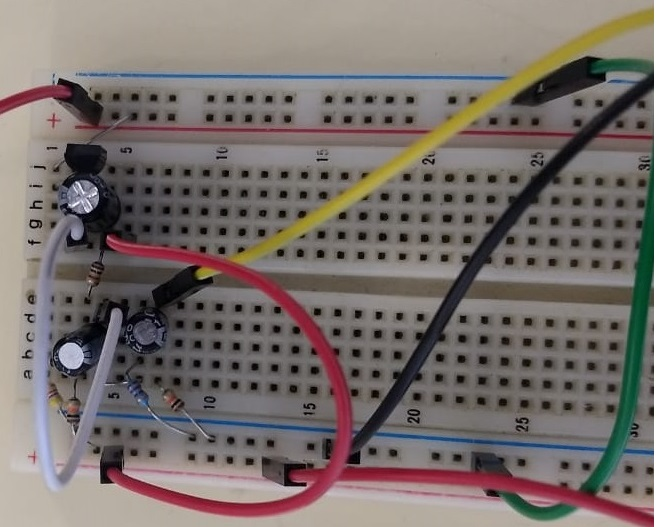
\includegraphics[scale=0.6]{imagenes/proto.jpeg} 
\caption{Circuito implementado en protoboard.}
\end{figure}

\subsection{Estimadores}

Una vez elegidos los valores de los componentes a utilizar, se calcularon los valores de los estimadores para el modelo incremental del transistor, siendo estos:

\begin{equation*}
\left\{
\begin{aligned}
	& \hat{hfe}=380 \\
	& \hat{hie}=4750\Omega \\
	& \hat{\frac{1}{hoe}} = 45k\Omega
\end{aligned}
\right.
\end{equation*}

\subsection{Resultados de Interés: Primer Ensayo}
Se calcularon los valores de la ganancia de tensión, corriente, impedancia de entrada y de salida para una $R_s=50\Omega$, siendo estos presentados a continuación:

\begin{equation}
	\Delta V_s \triangleq \frac{V_o}{V_s} = 0.99
\end{equation}
\begin{equation}
	\Delta i_s \triangleq \frac{i_o}{i_s} = 9
\end{equation}
\begin{equation}
	R_{is} = 91k\Omega
\end{equation}
\begin{equation}
	R_{os} = 867.65\Omega
\end{equation}

Luego se graficó la ganancia de tensión en función de la frecuencia:
\begin{figure} [H]
	\centering
	\includegraphics[width=0.9\textwidth]{imagenes/avs.png}
	\caption{Transferencia Módulo.}
	\label{fig:transmod}
\end{figure}

\begin{figure} [H]
	\centering
	\includegraphics[width=0.9\textwidth]{imagenes/avsp.png}
	\caption{Transferencia Fase.}
	\label{fig:transph}
\end{figure}

Una cualidad a notar es que esta configuración tiene una ganancia de tensión menor a 1 y que, para el rango de frecuencias utilizadas, el circuito se comporta como un pasa-altos, si bien realmente, al continuar aumentando la frecuencia, eventualmente decaerá en un pasa-banda aún así despreciando las puntas del osciloscopio y capacitancias parásitas del protoboard. Esto se debe al efecto de las capacitancias internas del transistor. Algunas posibles aplicaciones para el circuito son las de amplificador de corriente o como seguidor de tensión. El circuito también es conocido como ``seguidor por emisor''.

Otro aspecto de interés se puede ver en la fase, dado a que el circuito no invierte a esta.
\begin{table}[H]
\centering
\begin{tabular}{cccc}
\hline                   & $\mathbf{\Delta V_S}$ & $\mathbf{R_{In}}$ & $\mathbf{R_{Out}}$ \\
\hline
\textbf{Simulación} & -0.078 [dB]          & 66.0 [$k\Omega$]    & 200 [$\Omega$]     \\
\textbf{Calculado}  & -0.077 [dB]            & 96.3 [$k\Omega$]   & 848 [$\Omega$]     \\
\textbf{Medido}     & -0.100 [dB]             & 83.4 [$k\Omega$]  & 570 [$\Omega$]   	\\
\hline
\end{tabular}
\caption{Comparación de valores obtenidos de diversos enfoques.}
\label{tabla:comparacion}
\end{table}



\subsection{Resultados de Interés: Segundo Ensayo}
Se repitió la experiencia con una resistencia $R_s = 10k\Omega$, obteniéndose los siguientes resultados:
\begin{equation}
\Delta V_s \triangleq \frac{V_o}{V_s} = 0.892
\end{equation}
\begin{equation}
\Delta I_s \triangleq \frac{I_o}{I_s} = 9
\end{equation}
\begin{equation}
R_{is} = 100.9k\Omega
\end{equation}
\begin{equation}
R_{os} = 9664.5\Omega
\end{equation}
A continuación se graficó la transferencia del circuito en módulo y fase:

\begin{figure} [H]
	\centering
	\includegraphics[width=0.9\textwidth]{imagenes/avs10k.png}
	\caption{Transferencia Módulo con $R_s = 10k\Omega$.}
	\label{fig:transmod}
\end{figure}

\begin{figure} [H]
	\centering
	\includegraphics[width=0.9\textwidth]{imagenes/avsp10k.png}
	\caption{Transferencia Fase con $R_s = 10k\Omega$.}
	\label{fig:transmod}
\end{figure}

Se puede observar como la respuesta en frecuencia del circuito posee un polo alrededor de $1MHz$. Esto se debe a las puntas utilizadas para medir el circuito, ya que la simulación sin el modelo de puntas del osciloscopio carecía de esta característica. Además, se observa como la transferencia medida discrepa de la simulada para altas frecuencias y esto se debe a los efectos capacitivos despreciados del transistor y a capacitancias parásitas del protoboard utilizado. 

Luego, se armó una tabla con las diferencias en las características de interés de ambos ensayos.

\begin{table}[H]
\centering
\begin{tabular}{cccc}
\hline $\mathbf{R_s}$ & $\mathbf{\Delta V_S}$ & $\mathbf{R_{is}}$ & $\mathbf{R_{os}}$ \\
\hline
\textbf{$50\Omega$} & 0.9903          & 91 [$k\Omega$]    & 867.65 [$\Omega$]     \\
\textbf{$10k\Omega$}  & 0.8927            & 100.9 [$k\Omega$]   & 9664.5 [$\Omega$]     \\
\hline
\end{tabular}
\caption{Comparación de valores interesantes obtenidos en ambos ensayos.}
\label{tabla:comparacion}
\end{table}

Como se puede observar, la ganancia del sistema empeoró en casi un 10\% mientras que la resistencia de entrada empeoró en más de un 100\%. Esto muestra como el circuito se comporta mucho más cercano al ideal cuanto más baja sea la impedancia de salida de la etapa anterior a la que esta conectado.

\section{Conclusiones}
Se puede observar como la ganancia de tensión atenúa pero no en gran cantidad. Además, la impedancia de entrada del circuito es muy alta mientras que la impedancia de salida es muy baja, resultando ser el circuito una muy buena opción para acoplar impedancias o como seguidor de tensión. 

Las impedancias de entrada y salida medidas son similares a las calculadas, pero no iguales. Estas variaciones se deben a efectos no considerados en el modelo del transistor. A pesar de ello no son realmente un problema, dado a que como la impedancia de entrada es grande en los 3 casos, y la de salida es pequeña se toman como válidos los resultados. 

Finalmente se destaca que el tipo de resultados obtenido era esperable ya que el circuito analizado es una modificación del colector común, siendo así los resultados obtenidos similares a los de dicha configuración.
\end{document}